\chapter{Use case: Next order prediction} \label{chapter:use-case}

One of the goals of this project is to integrate an artificial intelligence solution within a CRM. After the analysis reported in chapter \textit{CRM AI}, it has been decided to develop a predictive machine learning model based on CRM data. This part if the thesis has been developed in collaboration with one of ELCA's client, hereafter referenced as \textit{Contoso} \footnote{Client's name and business subject to confidentiality.}.

This chapter details the entire machine learning project. Sections \ref{sec:use-case} and \ref{sec:ml-metrics} explain the business problem \textit{Contoso} is currently facing and how a machine learning solution might solve it. The data contained in Contoso's CRM is explained in section \ref{sec:crm-data} and section \ref{sec:ml-experimentation} details the machine learning experimentations based on this data. The deployment and integration with Contoso's CRM of the model created are outlined in section \ref{sec:crm-deployment}. Finally, sections \ref{sec:use-case-further-work} and \ref{sec:use-case-conclusion} conclude the chapter with a reflection on the entire initiative.

% -------------------------------- Section: Client's use case
\section{Client's use case} \label{sec:use-case}
\textit{Contoso} is an energy-focus enterprise active overall Switzerland offering several products and services. One of their product is subject to a very tense market, where its characteristics are the same among all competitors in the market with the price as the only differentiator. When dealing with this product, several of its specificities must be taken into account:
\begin{itemize}
\item The product is classified as a \textit{safety need} in Maslow's \textit{hierarchy of }needs\cite{wiki:Maslow's_hierarchy_of_needs}, meaning that people don't buy it because the \textit{like} it but because they \textit{need} it. 
\item Due to its classification in Maslow's hierarchy, the product is usually stored in high quantities. The typical customer will make a large order, fill its supplies, consume the product and once fully consumed, the product is bought again in large quantities. Therefore, the product is not bought on a daily basis but rather on an annual basis. This is a real difficulty for Contoso while trying to build customer loyalty.
\item Since the product's characteristics are the same for the entire market, the price is the only variable that companies can \textit{play} with. Nevertheless, part of the price is subject to global market variation, from which companies will adapt their margins. As all stock market, the prices can vary, even marginally, each day.
\end{itemize}

 Based on these particularities, building a solid customer relationship is difficult for Contoso: Customers only need to make one order per year in average and they are usually not subject to an immediate need. Therefore, they can take the time to compare the price offered by all suppliers in the market and make an order accordingly. This explains why Contoso is facing a high customer turnover and often dealing with \textit{one-time customers}, as shown by figure \ref{fig-annex:orders_per_accounts}.
 
 
 To dwindle customer churn and get lost clients back, \textit{Contoso} is building \textit{customer recovery} plans and reinforcing interactions with other products and services to form a complete ecosystem, but they want something uniquely targeting their key-product. Currently, Contoso's marketing team are contacting clients with annual newsletters. Those newsletters are sent to each client every year around the same period. The company wants to strengthen this marketing process by reaching out to clients at the perfect time, juste before they start to search for offers from the competition. This will enable Contoso to retain clients and ultimately build customer loyalty.
 
 
% -------------------------------- Section: Project outline
\section{Formalize machine learning problem} \label{sec:ml-metrics}

As defined in section \ref{sec:use-case}, the goal of this initiative is to build a machine learning model that predicts the time of a customer's next order. This problem can be formalize as a regression problem, for which the machine learning model will output the date of next order: at date $d$, the model will predict $i$, the number of days until next order. So $d+i$ will give the precise data of customer next order. Variants are to define $i$ as the number of weeks or months until next order. The date will be less precise but the predictions might turn out to be more satisfying. Another possibility is to formalize it as a classification task and output a binary value to the question : \textit{"Will this customer make an order in the coming day/week/month ?"}. After discussion with \textit{Contoso}, it has been decided to define the output of the model as \textit{the number of months until customer next order}. In details, it has been decided first to work with regression models to have multiple ranges of outputs. Then, for the output's granularity (day, week or month), predicting the number of month until next order \textit{should} give stronger results. It will allow \textit{Contoso} to asses how well a regression techniques are suited for this problem and, in a second phase, trying to have more precise predictions, with an output at the week level for example.

From the machine learning output, Contoso wants to reach customers before they make an order. The process is planned as follow:
\begin{enumerate}
    \item At the beginning of each month, compute the predictions for all active clients\footnote{An client is flagged as inactive if no more business can be made with him/her (moving abroad or death for example)}.
    \item Retrieve all clients with a predictions smaller than $2$.
    \item Get in touch with these clients if and only if they have not been contacted in the past two months.
\end{enumerate}
The last step of this process is very important, as it will ensure that the company won't reach the same client twice.


Now that the machine learning goal and usage have been specified, the metrics for its success must be defined. As stated above, this is a regression model, where the output will be a real number. Usual metrics for regression problems like Mean Absolute Error (MAE) or Root Mean Squared Error (RMSE) are not well suited for this project and for the usage of the predictions by \textit{Contoso}. As specified above, the company plans to get in touch with a client only if the predictions is below $2$. Therefore, if the output of a model is equal to $7.0$ months or $4.35$, it ends up being the same for \textit{Contoso}. This explains why RMSE or MAE cannot be used to evaluate machine learning models performance. As regression metrics are not applicable, the models will be assess with custom metrics inspired by classification problems: precision, recall and F1 score. 

To transform the regression problem into a classification one, model's predictions will be classify into one of the following four classes: \texttt{0, 1, 2 or 3+}. The class \texttt{0} is meant for predictions between 0 and 1 (excluded) - clients that should make an order in the current month. Same idea for classes \texttt{1} and \texttt{2}. The class \texttt{3+} regroups all predictions with an output bigger or equal to 3 - client next order should occur in three or more months.

\begin{adjustwidth}{-1cm}{}
    \begin{minipage}[b]{0.60\linewidth}
    \resizebox{1.0\columnwidth}{!}{
        \begin{tabular}[t]{c|c|
                >{\columncolor[HTML]{EFEFEF}}c|c|
                >{\columncolor[HTML]{EFEFEF}}c }
                Customer & y\_true & y\_true class & y\_pred & y\_pred class \\ \hline
                A        & 2       & 2             & 3.32    & 3             \\
                B        & 0       & 0             & 0.4     & 0             \\
                C        & 0       & 0             & 0.1     & 0             \\
                D        & 5       & 3+            & 2.9     & 2            \\
                E        & 3       & 3+            & 0.8     & 0             \\
                F        & 1       & 1             & 1.6     & 1             \\
                G        & 1       & 1             & 0.8     & 0             \\
                H        & 2       & 2             & 1.4     & 1             \\
                I        & 9       & 3+            & 15.2    & 3+            \\
                J        & 0       & 0             & 2.5     & 2            
        \end{tabular}
        }
        \captionof{table}{Example of output truth and predictions}
        \label{table:example_truth_preds} 
    \end{minipage}
    \hspace{1.0cm}
    \begin{minipage}[b]{0.45\linewidth}
        \offinterlineskip
        \moveright 1cm \hbox{\raisebox{1.8cm}[10pt][10pt]{\rotatebox[origin=c]{90}{\parbox[c][0pt][c]{15cm}{True class\\[50pt]}}}\par}
        \hspace*{1cm}\MyHBoxT[\dimexpr5.1cm]{Predicted class}\vspace*{-0.4cm}
        \hspace*{1cm}\MyHBox{0}\MyHBox{1}\MyHBox{2}\MyHBox{3+}\vspace*{-0.2cm}
        \MyTBox{0}{2}{0}{1}{0}
        \MyTBox{1}{1}{1}{0}{0}
        \MyTBox{2}{0}{1}{0}{1}
        \MyTBox{3+}{1}{0}{1}{1}
        \captionof{table}{Confusion matrix for table \ref{table:example_truth_preds}}
        \label{table:example_confusion_matrix} 
    \end{minipage}
\end{adjustwidth}


Based on this classes assignment, a confusion matrix can be generated. Then, custom metrics inspired by precision, recall and F1-score are computed:
\begin{itemize}
    \item \textbf{Precision}: Of all clients that make an order in the current month, how many where predicted with class 0 or 1? This metric computes the percentage of true orders catch by the model. 
    $$ Precision = \frac{t_0\_p_0 + t_0\_p_1}{t_0\_p_0 + t_0\_p_1 + t_0\_p_2 + t_0\_p_{3+}} $$
    
    For the example in table \ref{table:example_confusion_matrix}, the precision is equal to $\frac{2+0}{2+0+1+0} = 0.667$
    
    \item \textbf{Recall}: From all clients that the model has predicted an order for the current month, how many did actually made an order in the current or coming month? The goal with this metric is to assert that the model is not always predicting 0, which will give a precision score of 100\%, but will make \textit{Contoso} contact all clients. 
    $$ Recall = \frac{t_0\_p_0 + t_1\_p_0}{t_0\_p_0 + t_1\_p_0 + t_2\_p_0 + t_{3+}\_p_0} $$
    
    For the example in table \ref{table:example_confusion_matrix}, the recall is equal to $\frac{2+1}{2+1+0+1} = 0.75$
    
    \item \textbf{F1-score}: Same as the F1-score for classification tasks. 
    $$ \fscore = \frac{2*Precision*Recall}{Precision+Recall} $$

    For the example in table \ref{table:example_confusion_matrix} the F1-score is equal to $\frac{2*0.667*0.75}{0.667+0.75} = 0.71$
\end{itemize}

In the formulas above, $t_i\_p_j$ correspond to the sum of true orders occurring in \texttt{i} months and predicted to occur in \texttt{j} months. For example $t_0\_p_0$ corresponds to the count of orders occurring in the current month and predicted as such (top left case in the confusion matrix).

The dataset will be divided into training, testing and validation sets. The training set is composed of data associated to orders that took place between 2013 and 2016 and will be used to train all models. Data related to orders that occured in 2017 form the testing set, use to test each model created. Finally, data that come from orders made from January 2018 to Juin 2018 are in the validation dataset, only used once to compute the final score.

The metric \textbf{F1-score} will be the benchmark metric for this project.

% -------------------------------- Section: Data
\section{Data from CRM} \label{sec:crm-data}

This section outlines the data gathering, cleaning, transformation and feature engineering processes. Before doing some machine learning experiments, a first goal is to understand the data and figure out the main factors that push a client to make an order. For the analysis of data and machine learning experiments, the development has been done within \textit{Jupyter Notebooks} with a \texttt{Python 3} kernel, mainly relying on the \textit{Pandas} package.

Data comes from \textit{Contoso} CRM, a Dynamics 365 Online instance. By using to the \textit{Web Api} offered by Dynamics 365, all entities of the CRM have been retrieved and analyzed. From the 291 entities present in the CRM, only a few are useful for this project: \texttt{Orders}, \texttt{Accounts}, \texttt{Contacts} and \texttt{Buildings}. The relationships between those entities are straightforward: An order must be linked to an account and each account is linked to at least one contact, one of which must be the \textit{primary contact}. The \texttt{Contact} entity models a real person, where the \texttt{Account} entity models a customer of \textit{Contoso}, either a person or a company. Contacts can then be linked to one or more instance of the \texttt{Building} entity.

\begin{figure}[h]
    \centering
    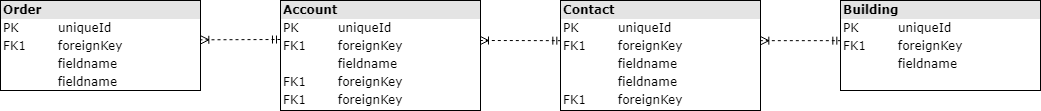
\includegraphics[width=15cm]{images/entityDiagram.png}
    \caption{Entity Diagram for \textit{Contoso} CRM data - \textbf{TODO}}
    \label{fig:entity-diagram}
\end{figure}

\subsection{Orders}\label{sec:crm-orders}

The \texttt{Order} entity holds all information about an order made by an account. The CRM contains all orders received by \textit{Contoso} since 2013 until nowadays. For this project, all orders considered ranged from January 2013 until June 2018, included. Once the raw data has been downloaded from all \texttt{Orders} entities, the first steps are to clean this set of 808'532 orders. Indeed, even if a CRM save its data in an organized manner and Dynamics 365 has some verification upon data entry, mistakes can still happen when a person enters data into the system. Orders have been discarded based on their names -empty or not-, on their status -active or not- and on their internal characteristics (amount delivered equal to zero, delivery date in 1956, delivery date occurring before the order date, ..). This cleaning phase removes 28.79\% of the orders, which gives a data set of 575'679 orders, each order having 37 features.

All these orders have been made by 183'706 accounts, with a mean of 3.14 orders per account and a median of 2. Grouping accounts per the number of orders made reveals that 50.77\% of accounts is this dataset have made one or two orders\footnote{Accounts which have made at least one order since 2013 - Figure \ref{fig-annex:orders_per_accounts} in the annexes.}. This demonstrates the singularity of a very competitive market in which clients often change their suppliers and fully benefit from the competition. In respect to the machine learning model, it will be very difficult to extract some common behavior and generalize, due to the low amount of orders for those accounts. Therefore, accounts with less than three orders have been discarded, leading to a dataset composed of 451'986 orders (-21.49\%).

As traditional accounts only order once per year, there is a seasonality effect visible when plotting the number of orders per month trough the years (figure \ref{fig:order_per_monthyear}). Even if the periodicity of orders isn't regular, a year experiences two pics of orders: one around March and another around October. On the opposite side, there have been fewer orders in Spring, around the month of June. The data plot in figure \ref{fig:order_per_monthyear} indicates that the weather must play a crucial order when accounts are making orders - it's colder in March and October than in June. As detailed in further section \ref{sec:external-data}, the model will take some weather-related information into consideration.

\begin{figure}[h]
    \centering
    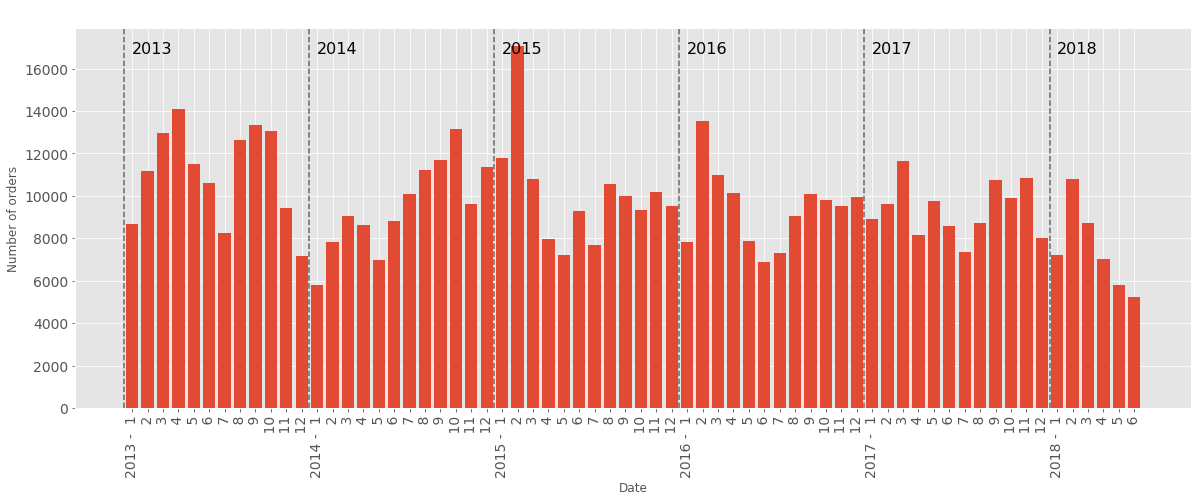
\includegraphics[width=15cm]{images/order_month_year.png}
    \caption{Number of orders per month per year}
    \label{fig:order_per_monthyear}
\end{figure}


As stated above, a typical customer will make an order once per year, with a number of months between two orders around 12 months, as presented in figure \ref{fig:orders-account-counts}. A mean of 12.67 months and a median of 11 months are retrieved by computing the average "wait" time between two orders for all accounts. Figure \ref{fig:orders-account-counts} shows that there is a lot of accounts waiting 11 months between two orders, but there is also account which order more frequently. On the other side, the number of accounts waiting 13 or more months between two orders decreases. Within this plot, there are two pics: the first one logically around 11 months and a second one around 23 months. This second pic is probably due to "jumper accounts", accounts that order one year with \textit{Contoso}, the following year with the competition and, two years after they first orders, order again with \textit{Contoso}. 

\begin{figure}[h]
    \centering
    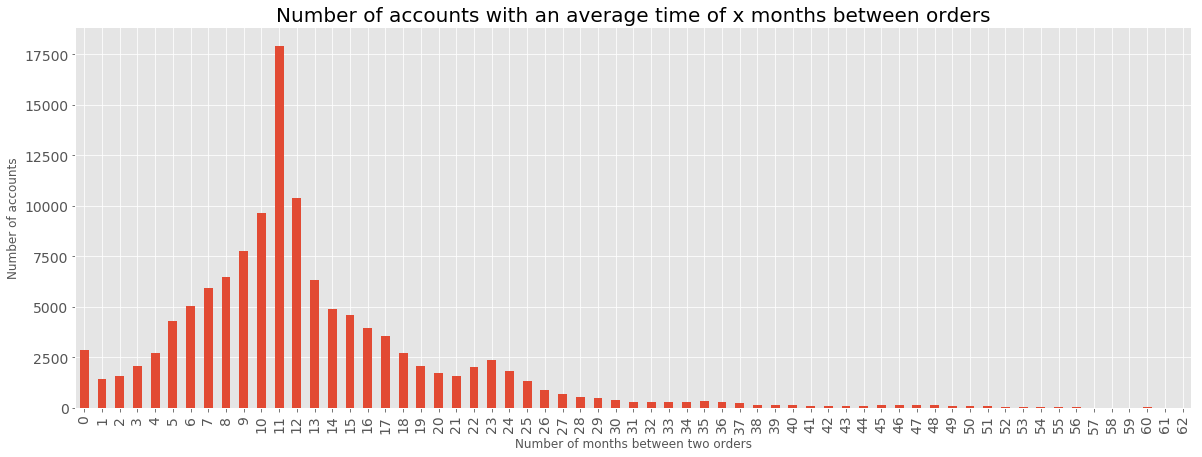
\includegraphics[width=15cm]{images/accounts-average-time-orders.png}
    \caption[Average number of months between two orders]{Accounts grouped by the average number of months between two orders}
    \label{fig:orders-account-counts}
\end{figure}

This plot also reveals \textit{key-accounts}, accounts ordering at least once per month. Those accounts are most of the time companies, considered as very regular customers by \textit{Contoso}. As detailed in section \ref{sec:data-shape-for-ml}, \textit{key-accounts} will not be a problem for the machine learning model.


\subsection{Accounts, Clients and Buildings}\label{sec:crm-accounts}
The \texttt{Account} entity holds information related to the clients of \textit{Contoso}, either a natural or legal person. Due to imports from a legacy system, the Dynamics 365 instance of \textit{Contoso} contains more than 1'100'000 accounts. Filtering those accounts based on the final orders from section \ref{sec:crm-orders} gives 88'552 accounts, with 244 features per account. The company stocks a lot of account properties in their CRM and the vast majority of those are null or not useful for this next order prediction task. After a review of all these features, only 11 will be kept, among which account's activeness and account's name, which will be compared to it's primary client name.

Indeed, all accounts are linked to a primary contact. The \texttt{Contact} entity holds information about a physical person, like its address or phone number. From this entity, only two features will be used: the birth date and the name. The birth date will be used to see if the age of a person as an influence on it's buying habits. The contact name will be use in comparison with the account name. As mentioned above, the \texttt{Account} entity can be a natural or a legal person, but there is no feature in the CRM to specify this account state. As this information is important -a legal person can make orders on a very frequent basis- such feature is built. An account's name can be compared to the name of its primary contact. If both names are equal, the account will be considered as a natural person, otherwise the account will be considered as a legal person, assuming that an account modelling a legal person will not have the same name as it's primary contact. As shown in figure \ref{fig:account-contact-name-orders}, accounts classified as a legal person made orders much more frequently.

\begin{figure}[h]
    \centering
    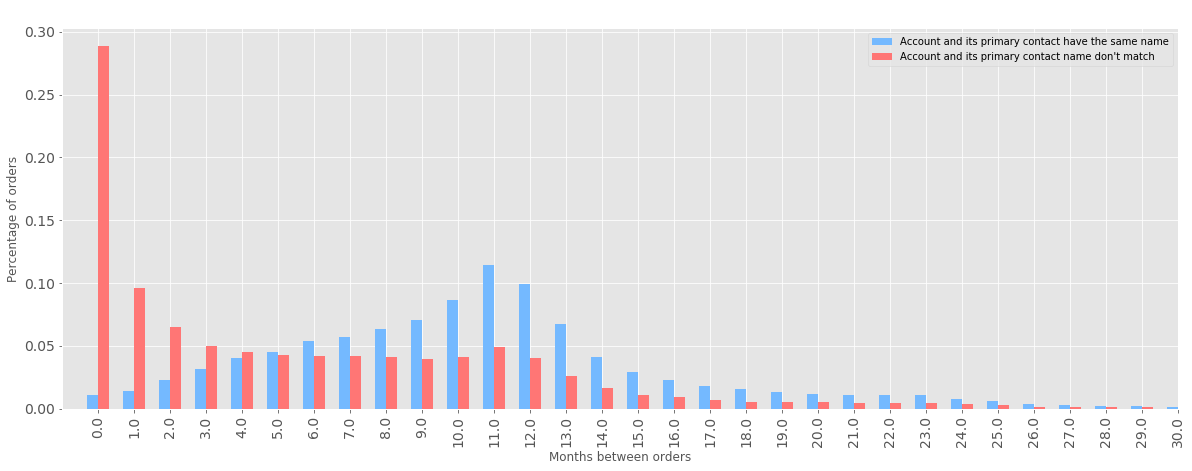
\includegraphics[width=15cm]{images/account-contact-name-orders.png}
    \caption[Account and contact's name influence of order's frequency]{Number of months between two orders related to the account-contact name}
    \label{fig:account-contact-name-orders}
\end{figure}

Regarding the \texttt{Building} entity, it holds information about the building of a contact (house, offices, cottage, ...). Even if not all contacts have such link (80.84\% of contacts are linked to at least one building), this entity will be used to build new features modeling the amount of product stocked and used, as detailed in section \ref{sec:ml-features}.


\subsection{External data}\label{sec:external-data}
In addition to the data coming from Dynamics 365, there are two important variables to take into account for predicting the date of customer next order: price and weather. This two datasets will be used to created new features, detailed in section \ref{sec:ml-features}.

As explained in section \ref{sec:use-case}, the prices are mainly dependant of the stock market, which can change every day. Therefore, it has been observed by \textit{Contoso} that when the price is going down, more orders are being made and when the price is going up, customers would rather wait a bit more, consume their stock and waiting for a decrease to place a new order. A dataset containing the monthly prices of \textit{Contoso} between 2013 and 2018 has been created. Unfortunately, it was not possible to compare this data with the monthly prices set by each competitors.

Weather data has also an influence on the ordering patterns of clients, as shown in section \ref{sec:crm-orders}. Weather data has been provided by \texttt{MeteoSwiss} with several daily metrics associated to the 20 meteorological station across Switzerland (weather, precipitations, wind, ...). Based on the primary contact address, each \texttt{account} object has been linked to one of those station and among all metrics, only the weather degrees \big[°C\big] have been used.


\section{Data for the machine learning}
Once that all data has been gathered, cleaned and analyzed, it needs to be shaped in such format that machine learning models can use it. This section detail how the data from \ref{sec:crm-data} has been combined and then reshaped to be given to machine learning models.

\subsection{Dataset construction}\label{sec:data-shape-for-ml}
As defined above, the model's output will be the number of months until customer next order and the model is planned to be used on a monthly basis. For all accounts, one entry per month is created, from the first month after client's first order until the month of last order. For all monthly entries, the output is the number of months until next customer order and the data contains features related to the account (shared among all entries), features related to the previous orders and features related to the current month, like the monthly weather for example. 

Figure \ref{fig:data-build-example} contains an example of such data creation process. Marked as yellow circles, this account has made four orders in April 2013, March 2014, January 2015 and March 2016. The first entry in the final ML dataset concerns May 2013, the month following account's first order. The output of this entry is set to 11 months, the number of months between May 2013 and April 2014, date of account's second order. The same principle will be apply to all following months, until March 2016, date of the last order made by this account.

\begin{figure}[h]
    \centering
    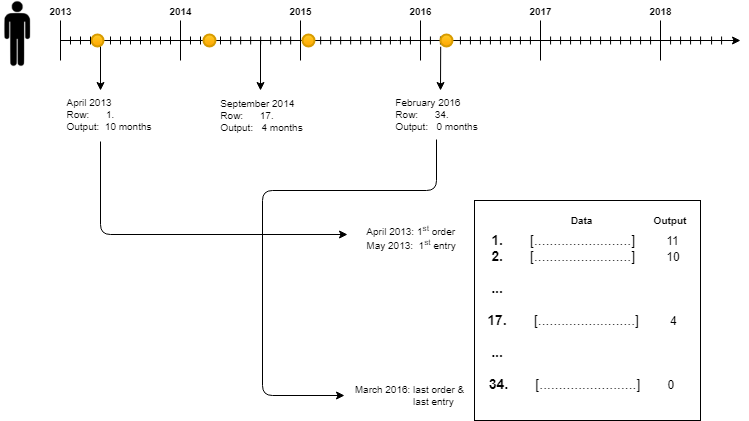
\includegraphics[width=14cm]{images/data-build-ml-example.png}
    \caption[Process to build data for machine learning]{Sketch of the ML model data building process. Yellow circles model account orders.}
    \label{fig:data-build-example}
\end{figure}


% -------------------------------- Section: Customer Jounrey + Feature engineering
\subsection{Feature engineering}\label{sec:ml-features}

Before creating new features, all datasets must be combined together. Starting for right to left on figure \ref{fig:entity-diagram}, \texttt{Building} and \texttt{Contact} data are combined since a contact may be linked to one or multiple building (one-to-many relation). From the \textit{Building} entity, only one feature will be used: the volume of its reservoir, used to stock the product. In the case of multiple buildings being linked to the same account, the average capacity of all reservoirs will be computed and added to the contact data. 

Then, the entities \texttt{Account} and \texttt{Contact} are combined based on the account primary contact, with its address and birth date added to the account. This combination of the \texttt{Account}, \texttt{Contact} and \texttt{Building} entities builds a first set of features, defined as \textit{account-related} features.

Each row in the final machine learning data is composed of three types of features: the \textit{account-related} ones, features related to the current month and features about the previous order. Features related to the current month are mainly build from the two external data to encapsulate the variations of the prices and the weather temperature through time. Finally, the previous order is also used to capture its characteristics, like "\textit{Was it a big or a small order}?" or "\textit{When did this order occurred compare to the one before?}".


\begin{figure}[h]
    \centering
    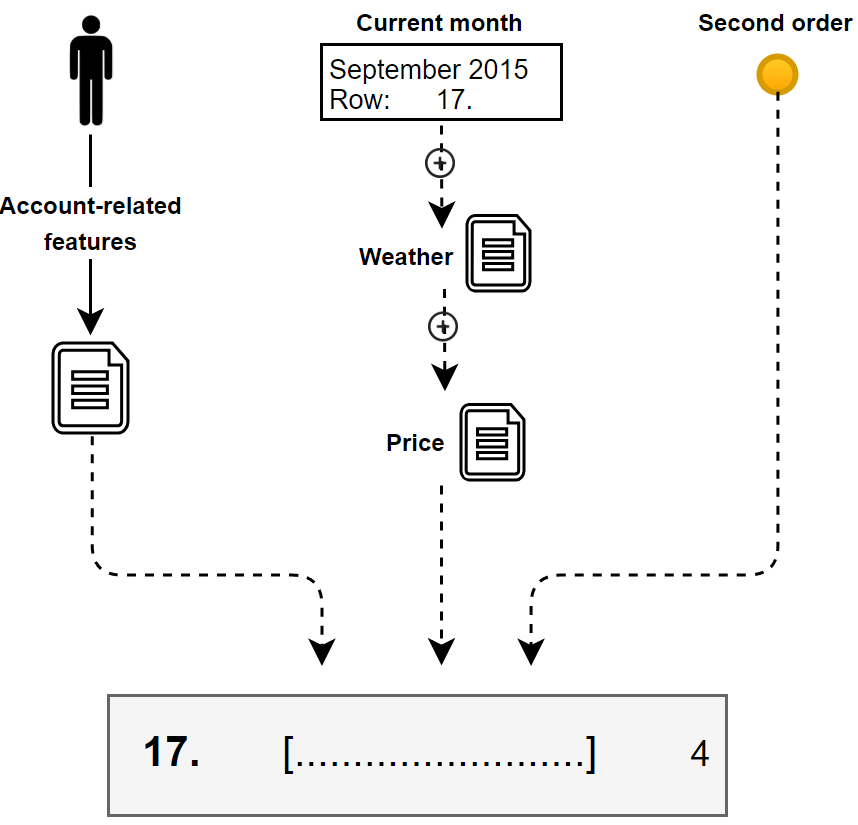
\includegraphics[width=8cm]{images/data-build-ml-example-row.png}
    \caption[Features building for specific month]{Sketch of the features used for the row of September 2014 in figure \ref{fig:data-build-example}}
    \label{fig:data-build-row-example}
\end{figure}

The exhaustive list of the 122 features build can be found in annex \ref{annex:features-for-ml}. Those features were created based on \textit{Contoso} knowledge of its business, meetings with the marketing team and analyses of \textit{Customer Journeys}. A \textit{Customer Journey} is a plot where all orders of a selected account are visible, with the \texttt{Weather} and \texttt{Price} information through the months (see an example in figure \ref{fig-annex:customer-journey}). 

Features were also created after a trial and error phase in the process of building and validating machine learning architectures. The property \texttt{feature\_importances\_} of \textit{Sklearn}'s models was also used to rank features and build new ones based on it.



% -------------------------------- Section: Machine Learning Experimentation
\section{Machine Learning Experimentation} \label{sec:ml-experimentation}

It is the first time Contoso is involved in a machine learning project with the goal to model its customer's behavior. As such, all types of models and architectures are possible. In this project, it has been decided to start with several types of models and a simple set of features. The first goal is to evaluate the feasibility of the task and the family of machine learning models best suited for it. 


\subsection{Models experiments}
Python' package \textit{Scikit-learn} was used to build the models of this section. Thanks to Scikit-learn offered ease for testing different models, several families of supervised learning models have been investigated, with results reported on table \ref{tab:scores-simple-models}. Among the models investigated, there are \texttt{Liner models} (linear regression), \texttt{Tree models} (extra tree and decision tree), \texttt{Ensemble models} (random forest, extra trees, gradient boost and bagging regressor) and \texttt{Neighbors models} (KNeighbors regressor).

In this initial phase, all models have been trained with scikit-learn's default parameters and a subset of 17 features manually selected\footnote{Those features are marked with an * in annex \ref{annex:features-for-ml}}. For all models created in this project, the same seed value has been used.

\begin{table}[!htb]
    \begin{tabular}{l|lll|lll}
                          & \multicolumn{3}{c|}{Train}                         & \multicolumn{3}{c}{Test}      \\
        \textbf{Model name}        & \textbf{Precision} & \textbf{Recall} & \textbf{F1-score} & \textbf{Precision} & \textbf{Recall} & \textbf{F1-score} \\ \hline
        Extra Tree        & 0.996     & 0.999  & 0.998                         & 0.324     & 0.389  & 0.354    \\
        Decision Tree     & 0.996     & 0.999  & 0.997                         & 0.267     & 0.394  & 0.318   \\
        KNeighbors        & 0.303     & 0.908  & 0.455                         & 0.131     & 0.508  & 0.208    \\
        Random Forest     & 0.696     & 0.998  & 0.820                         & 0.046     & 0.829  & 0.088    \\
        Bagging Regressor & 0.699     & 0.998  & 0.822                         & 0.045     & 0.829  & 0.084    \\
        ExtraTrees        & 0.996     & 0.999  & 0.998                         & 0.044     & 0.829  & 0.083    \\
        Linear Regression & 0.011     & 0.187  & 0.021                         & 0.028     & 0.305  & 0.051    \\
        Gradient Boosting & 0.000     & 0.000  & 0.000                         & 0.000     & 0.000  & 0.000    \\
    \end{tabular}
    \caption{Prediction scores for first models, ranked by their F1-score on testing set}
    \label{tab:scores-simple-models}
\end{table}

The first observation is that F1-scores aren't high and more than half of the models have a score below 0.10. It's also noticeable that all models are overfitting too much, except for the linear regression. The two tree models are giving the best predictions, with a good trade-off between precision and recall, where the ensemble models are very confident in their predictions (recall score above 80\%), but too cautious and catch less than 5\% of the orders.

The next experiments are related to the set of features used. With the predictions based on \texttt{Extra Tree} models, several features selection techniques have been used: Univariate selection where features are scored with the \textit{f\_regression}, Principal Component Analysis (PCA) and feature importance based on an \textit{ExtraTrees} model. The best F1-score turned out to be obtain with six features selected through the \textit{ExtraTrees} model. With a score of \texttt{0.636}, the model trained with only six features achieves a score almost twice as good as the one obtain previously. It's noticeable that the model gives it's better predictions when using a small number of features, as reported in figure \ref{fig:feature-selection}.

\begin{figure}[!htbp]
    \centering
    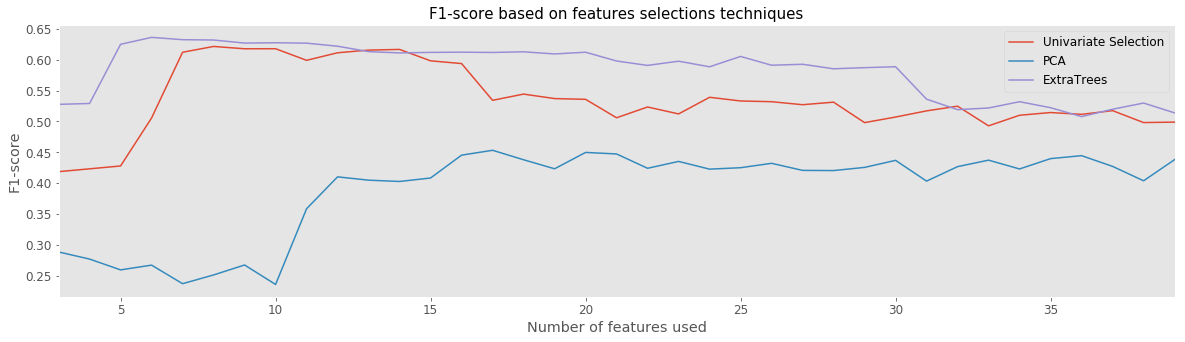
\includegraphics[width=15cm]{images/feature_selection.png}
    \caption[F1-score based on feature selection]{F1-score obtain on testing set with three different strategies for features selection}
    \label{fig:feature-selection}
\end{figure}

After optimizing the set of features, \textit{ExtraTree} regressor's internals parameters can also be optimized. The primary goal is to reduced the overfitting produced by the tree. Two parameters have been fined-tuned: \texttt{max\_depth} and \texttt{min\_samples\_split}. The \texttt{max\_depth} parameter has no value by default, therefore the tree expand itself until all leaves are pure, explaining the overfitting on training data. The \texttt{min\_samples\_split} parameter controls the minimum number of samples required for a node to be split at the depth level below. Most relevant results of this fine-tuning phase are reported in table \ref{tab:tree-fine-tune}.

\begin{table}[!htbp]
    \centering
    \begin{tabular}{c|c|c|c}
    \textbf{Max depth} & \textbf{Min samples split} & \textbf{Training F1-score} & \textbf{Testing F1-score} \\ \hline
    30	&  70   &  	0.738  &  0.715 \\
    50	&  100  &  	0.729  &  0.713 \\
    80	&  100  &  	0.729  &  0.713 \\
    30	&  100  &  	0.730  &  0.711 \\
    30	&  50   &  	0.748  &  0.710 \\
    50	&  70   &  	0.739  &  0.710 \\
    80	&  70   &  	0.739  &  0.710 \\
    50	&  50   &  	0.749  &  0.707 \\
    80	&  50   &  	0.749  &  0.707 \\
    30	&  10   &  	0.828  &  0.696 \\
    50	&  10   &  	0.854  &  0.683 \\
    80	&  10   &  	0.854  &  0.683 \\
    10	&  100  &  	0.449  &  0.466 \\
    10	&  10   &  	0.470  &  0.396 \\
    10	&  50   &  	0.439  &  0.388 \\
    10	&  70   &  	0.378  &  0.364 
    \end{tabular}
    \caption{F1 scores for training and testing data. Parameters tested are the \texttt{max\_depth} and \texttt{min\_samples\_split}. Table sorted by decreasing testing score.}
    \label{tab:tree-fine-tune}
\end{table}

With the best combination of \texttt{max\_depth} and \texttt{min\_samples\_split}, the model reaches a F1-score of 0.715 with the testing data. It's also noticeable that the model is not overfitting anymore, with similar results on the training data.


Alongside with experiment models and new parameters, optimizing the data to train model has been experiment. Until now, data-related optimization have only concern the features set, but there are some others possibilities. By investigating the data, three possible ways to reshape it were found. 
The first one consist of reducing the data by removing entries related to accounts with less than five entries. Then, for the remaining accounts, take only five random entries. The goal is to reduce the potential influence of accounts ordering very often and also reduce the potential noise in the data bring by accounts with very few entries. A second attempt to reduce the influence of \textit{extreme} accounts is to simply remove all accounts ordering every month or every two months. The third and last experiment to reshape the data is to have the same number of entries per output, in an attempt to standardize the output. All this three attempts to reshape the data never improved the F1-score previously obtained.

To summarize this section about experimenting several models available with \textit{Scikit-learn}, the best model is an \textit{ExtraTree} regressor which after a fine-tuning phase outputs predictions with a \textbf{F1-score of 0.715}.

\subsection{Neural Networks}
The \textit{ExtraTree} model has a big flaw: it's only using six features and none about weather or product's price. When trying to add those kind of features, the model wasn't as efficient as before. Therefore, a new type of machine learning model has been investigated: Neural Networks. Build with the Keras framework, six different architectures of Neural Networks have been experimented, all based on fully-connected layers. Similar to what has been done with previous models, several set of manually selected features have been used. The model achieving the best F1-score is a complete model composed of five fully-connected hidden layers trained with a set of 22 features and scoring \texttt{0.811} with the test data. All results and details of models tested are reported in annex \ref{annex:nn-experiments}.

Once that the model architecture has been chosen, internal parameters of the model can be investigated. Four parameters deserve some attention: the training \texttt{batch size}, model's compiler \texttt{loss function} and \texttt{optimizer} and the hidden layers \texttt{activation} function. Due to all possible values for those parameters, the fine-tuning phase has been done sequentially: starting from the baseline model of previous phase (table XXX-annex), first optimize the training batch size, then the activation function of hidden layers, model's compiler loss function and finally the model compiler (results reported in annex \ref{annex:nn-fine-tuning}). Parameters of the model obtained are outlined in table \ref{tab:nn-final-parameters}.

\begin{table}[]
    \centering
    \begin{tabular}{l|l|l}
        \textbf{Model part}           & \textbf{Parameter}                 & \textbf{Value}         \\ \hline
        Training                      & Number of epochs                   & 8                     \\
                                      & Input dimension                    & (X,22)                     \\ \hline
        Hidden layers                 & Number of neurons                  & 200-100-30                     \\
                                      & Activation function                & selu                     \\
                                      & Use bias                           & No                     \\ \hline
        \multicolumn{1}{l|}{Compiler} & \multicolumn{1}{l|}{Loss function} & \multicolumn{1}{l}{msle} \\
        \multicolumn{1}{l|}{}         & \multicolumn{1}{l|}{Optimizer}     & \multicolumn{1}{l}{adam}
    \end{tabular}
    \caption{Neural Network parameters for training final model}
    \label{tab:nn-final-parameters}
\end{table}


\subsection{LSTM}
A flaw present in previous models is that they are not account specific. Of course there are some account-specific features, but those are not enough to catch some use case. Let's assume that an account has a specific ordering strategy: make a big order in June, then make a new but smaller order in September and repeating the same ordering strategy each 15 months. For such account, the previous model will most probably not be able to catch its behavior with the features used. That's the main motivation for using Long Short-Term Memory (LSTM) networks in this project. Being part of the Recurrent Neural Networks (RNN) family, LSTMs have the ability to recognize patterns in sequences of data. This is a different problem compared to other types of supervised learning as sequences impose an order on observations.

To be able to use LSTMs, the data need to be reshaped. Previous models were expecting two-dimension input, but LSTMs required data to be in three-dimensions form: \texttt{[batch size, time steps, hidden size]}. To reshape the data, all entries related to the same account have been sorted by month and year (as detailed in section \ref{sec:data-shape-for-ml}, all entries are \textit{linked} to a given month). Among all these entries, one has been taken randomly and will be consider as the last \textit{step} of the LSTM data, while all entries occurring before will be considered as previous steps. Figure \ref{fig:lst-data-build} sketch this process. In order to have a dataset that a computer can still handle, the LSTM data is composed of a maximum of five entries per account and each entries has a maximum of 15 steps (15 monthly data).

\begin{figure}[!htbp]
    \centering
    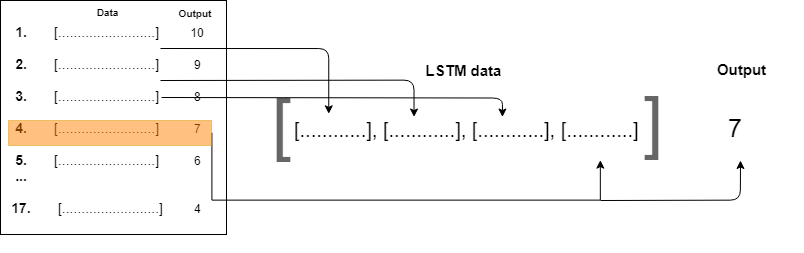
\includegraphics[width=10cm]{images/lstm-data-build.png}
    \caption[LSTM data build]{Example of reshaping the data for LSTM models. From the initial data, the fourth entry has been selected randomly and is placed as the last step of the data.}
    \label{fig:lst-data-build}
\end{figure}

Similar to the experiments with previous neural networks, several model architectures have been used to train LSTMs: one with only the LSTM layer, others with some fully-connected dense layers after the LSTM one. With the first experiments, results were similar to the one obtained with only fully-connected layers but on the batch size fine-tuning phase, results didn't improve the testing F1-score. Results are available in annex \ref{annex:lstm-experiments}.



\subsection{Best model evaluation}

The best model is a Neural Network composed of three fully connected hidden layers with 200, 90 and 30 neurons. Trained with the parameters reported in table \ref{tab:nn-final-parameters}, it achieves the following scores:

\noindent\hspace*{0.8cm}  1. \texttt{Training data}:   F1-score of \textbf{0.XXX}, precision of 0.XXX and recall of 0.XXXX \\
\hspace*{0.8cm}           2. \texttt{Testing data}:    F1-score of \textbf{0.XXX}, precision of 0.XXX and recall of 0.XXXX \\
\hspace*{0.8cm}           3. \texttt{Validation data}: F1-score of \textbf{0.XXX}, precision of 0.XXX and recall of 0.XXXX

As explained in section \ref{sec:ml-metrics}, this is a regression problem, but scored with metrics used for classification tasks. The confusion matrix for the validation data is presented in figure XXX.

\begin{figure}[!h]
    \centering
    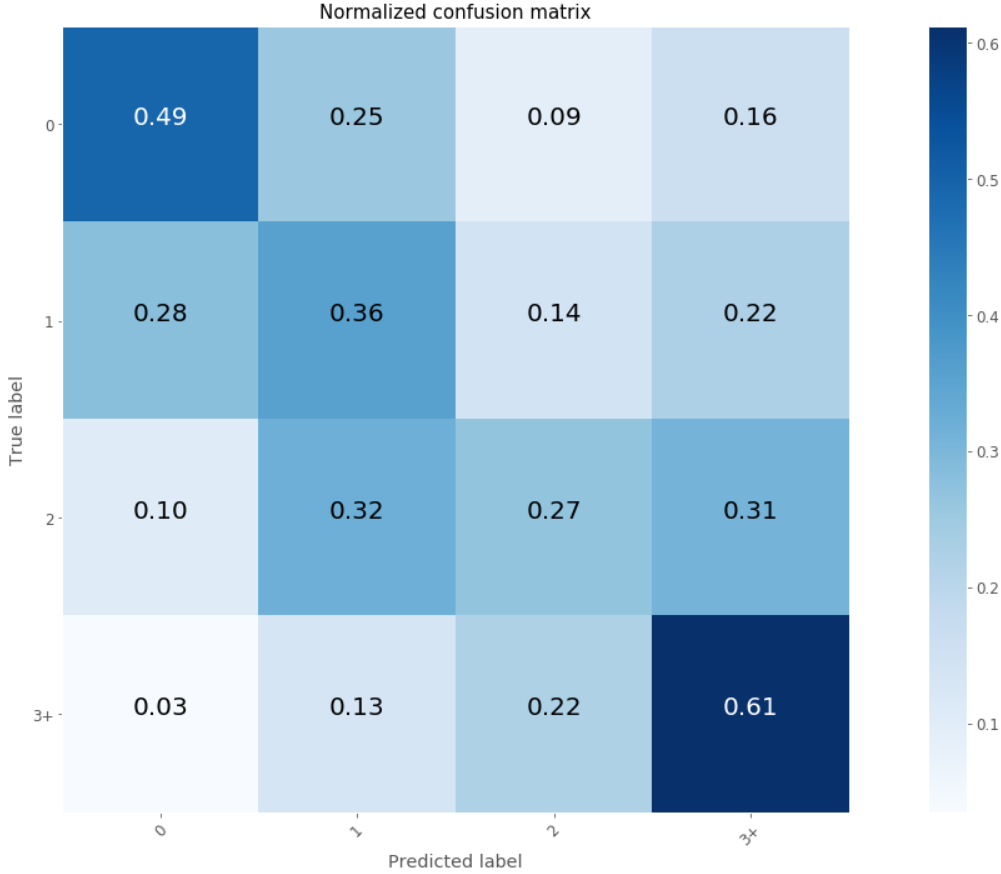
\includegraphics[width=7cm]{images/cf-matrix-validation.png}
    \caption[Confusion matrix for validation data]{Confusion matrix for the validation data obtain with the best model}
    \label{fig:lst-data-build}
\end{figure}


% -------------------------------- Section: Deployment
\section{Deployment} \label{sec:crm-deployment}
Once the final machine learning model has been build and tested, its results must be integrated within the Dynamics 365 instance of \textit{Contoso}. The end goal is to have a prediction for each account regarding the date of the next order. For this, two ways to make account predictions were defined:
\begin{itemize}
    \item Run the predictions every first Saturday for every month
    \item Run the predictions for a specific account directly for the CRM interface, at anytime.
\end{itemize}

Both integration will be supported by \textit{Azure} services.

\subsection{Azure Architecture}
To deploy the model, four Azure cloud services are used: Functions, Queue Storage, Web App and Application Insights. Azure Functions enable to run code on a serverless architecture and for it to be scaled, the Azure Queue Storage is a service to store large number of messages to be consumed via HTTP call, Azure Web App creates web application with built-in autoscale and Azure Applications Insights is used to analyze performances, errors and logs messages. The connection between those services and Dynamics 365 are sketch in figure \ref{fig:azure-deployment}.

\begin{figure}[!h]
    \centering
    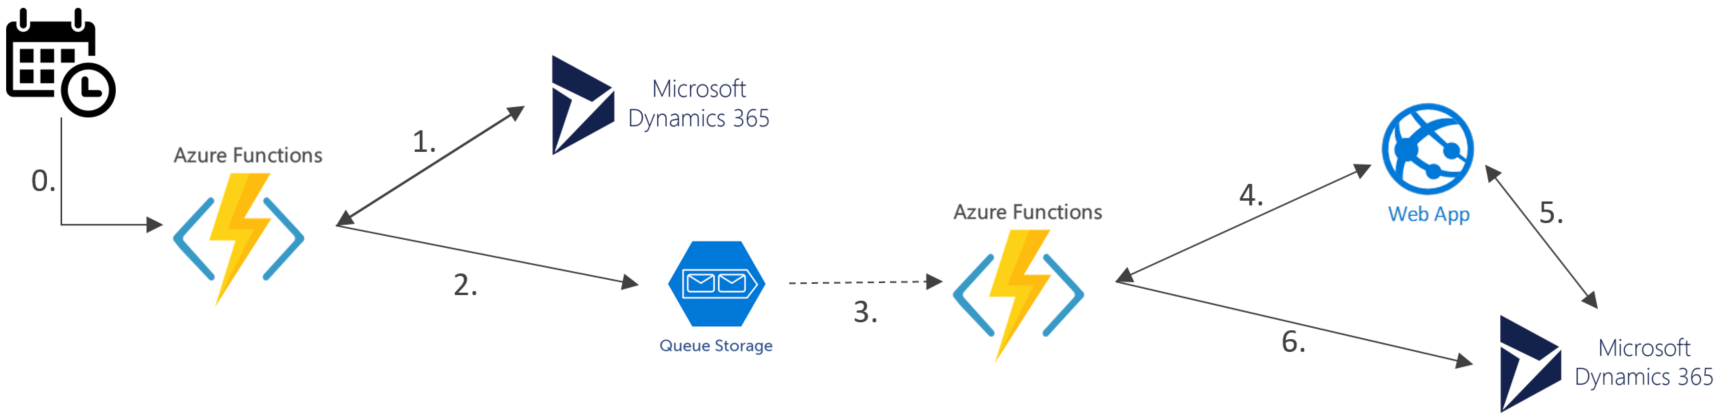
\includegraphics[width=12cm]{images/azure-archi-weekly.png}
    \caption[Deployment architecture for scheduled predictions]{Connection between Azure services and Dynamics 365 to compute predictions on a recurring basis.}
    \label{fig:azure-deployment}
\end{figure}

\noindent The architecture used to integrate machine learning predicitons inside Dynamics 365 contains the further steps:
\vspace*{-\baselineskip}
\begin{enumerate}[label=\texttt{\arabic*.}]
    \setcounter{enumi}{-1}
    \item The first Saturday of each month, at 03:00, the entire process is triggered.
    \item A first Azure Function will retrieve all accounts for Dynamics 365, via the Web Api. Only active accounts with at least three orders are retrieved.
    \item Once all accounts have been retrieved, they are added into a queue stored as an Azure Queue Storage.
    \item A second Azure Function is trigger each time new items are added into the Azure Queue Storage. This function will retrieve five accounts per run.
    \item The Azure Function retrieves the predictions for the five accounts with an HTTP request to the Web App.
    \item The Web App holds the entire logic of the prediction. Build in Python, it makes used of the \textit{Flask} microframework to create HTTP endpoints. When the Web App receives the accounts for the Azure function, it will connect to the CRM and build the data to give to the machine learning model. This model is stored in the Web App and used against the data just created. Predictions are then returned to the Azure Function.
    \item Once the Azure Function gets the predictions, it updates the CRM.
\end{enumerate}

One advantages of using this architecture is the connection between the Azure Queue Storage and the second Azure Function. It enables accounts to be consumed at a desired pace, in such a way to not overload the others components (Web App and CRM), to make the predictions before reaching the built-in of timeout Azure Functions and also to have another queue containing failures. In case of an error during the process, accounts for which the predictions weren't computed are added to a queue, in such way that they do not stop the entire process. For each step, Azure Application Insights are used to store logs.

Experiments with this architecture showed a total running time of approximately 8 hours for more than 100'000 accounts. Compared to others services powered by Azure like the \textit{Azure Machine Learning}' suite, this architecture is significantly less expensive, much more flexible and better suited for this use case.

The Azure Web App described above is also used to run the prediction for a specific account, upon CRM's user request. In that case, a JavaScript file stored in a Dynamics 365 Web resource is sending an HTTP request to the Web App, which computes the prediction.

\subsection{Integration with Dynamics 365}
The predictions made by the machine learning model must be visible and usable directly from Dynamics 365. Inside the \textit{Account} entity page, a section \texttt{ML Predictions} was created with two fields: Next Order Prediction and Last refresh. The first field contains the predicted month of accounts next order and the date of when was the machine learning model run is displayed below. This allow CRM users to see the prediction and when it was made. If the prediction is \textit{too old} or that new account-related information have been added, predictions can be refreshed on-demand, by clicking the blue button \textit{Run predictions}. This button will be grayed out and inactive throughout the entire process (~ 5-10 seconds). No refresh or page reload is necessary, both fields will be updated automatically. If the process ends successfully, the button will turn out green, but if a mistake happened, the button will be red.

\begin{figure}[!h]
    \centering
    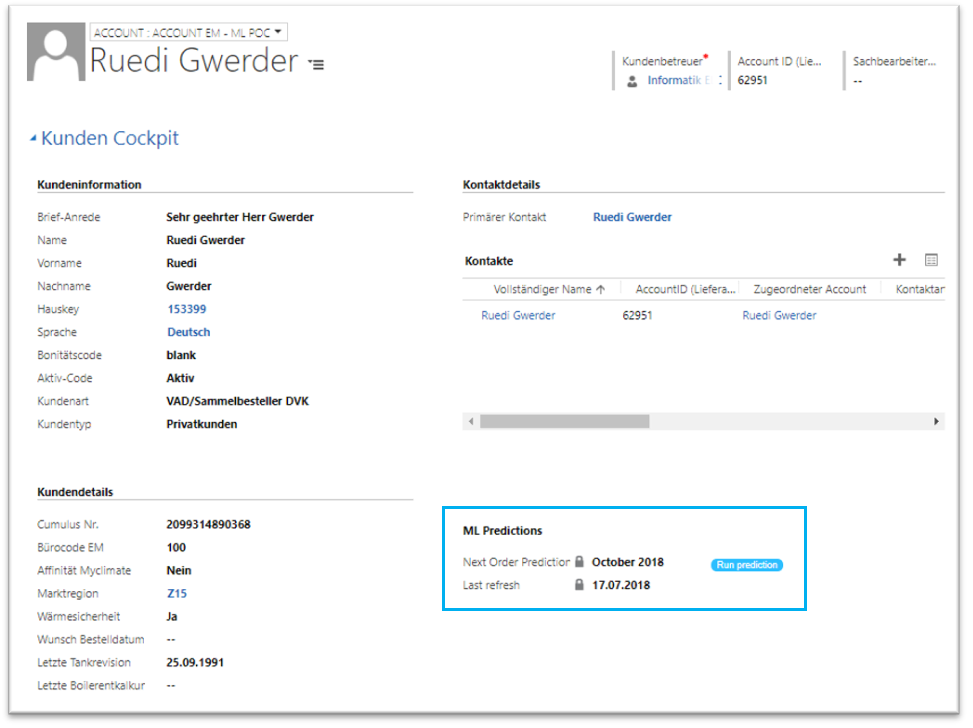
\includegraphics[width=12cm]{images/dynamics-account.png}
    \caption[Dynamics 365 \textit{Account} entity page]{Dynamics 365 Account entity page. The part related to the model predictions is in the blue rectangle. It contains two fields: \texttt{Next Order Prediction} and \texttt{Last refresh}, as well as a button \texttt{Run prediction}.}
    \label{fig:dynamics-account-ml-screenshot}
\end{figure}

As the prediction is stored as a CRM field, it can be used to create Marketing lists. In Dynamics 365, creating a marketing list is usually the first step in a marketing campaign. For Contoso use case, a marketing list containing all accounts with the field \textit{Next Order Prediction} happening in current or coming month can be created as a first step to contact accounts before they make an order and investigate competitor's offers.


% -------------------------------- Section: Further Work
\section{Further Work} \label{sec:use-case-further-work}



% -------------------------------- Section: Conclusion
\section{Conclusion} \label{sec:use-case-conclusion}